% Chapter 3

\chapter{Methodology}

\label{Chapter3} 

%----------------------------------------------------------------------------------------

\newcommand{\keyword}[1]{\textbf{#1}}
\newcommand{\tabhead}[1]{\textbf{#1}}
\newcommand{\code}[1]{\texttt{#1}}
\newcommand{\file}[1]{\texttt{\bfseries#1}}
\newcommand{\option}[1]{\texttt{\itshape#1}}

%----------------------------------------------------------------------------------------
\section{DFT calculations}

\subsection{History of density functional theory}

Density functional theory (DFT) is one of the most widely used methods in computational chemistry and materials science. It allows the efficient calculation of electronic structures for molecules and materials. Although DFT's conceptual foundation originated in quantum mechanics, it was formally established in the mid-20th century~\cite{DFT_Origins}.

In 1964, Hohenberg and Kohn demonstrated that the ground-state properties of a many- electron system depend entirely on its electron density, rather than on the complex many-body wavefunction \cite{Hohen_Kohn}. This significantly simplified the problem because electron density depends on only three spatial coordinates.

The following year, Kohn and Sham introduced the Kohn-Sham (KS) equations \cite{Kohn_KS_equations}, reformulating the many-electron problem as a system of non-interacting particles. Electron-electron interactions are incorporated through an exchange-correlation functional. Since the exact form of this functional remains unknown, various approximations have been developed over time. The first widely used functional was the Local Density Approximation (LDA), followed by more accurate methods, such as the Generalized Gradient Approximation (GGA) and hybrid functionals that incorporate Hartree-Fock exchange.

Despite its success, DFT still faces notable limitations. Accurately describing strongly correlated materials, van der Waals interactions, and excited states remains challenging. Standard DFT functionals often have difficulty with systems in which electron correlation plays a significant role, such as transition metal oxides \cite{DFT_strongly_correlated}. Additionally, conventional DFT approaches may inadequately capture dispersion forces, leading to inaccuracies in systems dominated by van der Waals interactions \cite{DFT_vdw_limitations}. Excited-state properties also pose difficulties, as time-dependent DFT (TDDFT) may fail to accurately describe certain excitation phenomena \cite{TDDFT_challenges}.

To address these challenges, ongoing research focuses on improving exchange-correlation functionals and integrating DFT with other computational methods. Researchers are actively pursuing strategies such as combining DFT with many-body perturbation theory (MBPT) and enhancing TDDFT techniques to overcome current limitations and expand the applicability of DFT to a broader range of complex systems \cite{DFT_MBPT_TDDFT}.


\subsection{Basis sets in quantum chemistry}

In this section, we provide a brief overview of the basis sets and functionals employed in this master's project.


Basis sets are fundamental to quantum chemical calculations, because they provide the mathematical functions used to approximate electronic wavefunctions. Since obtaining  exact solution of the Schrödinger equation for many-electron systems is generally infeasible, basis sets enable molecular orbitals to be expressed as linear combinations of predefined functions. This balances computational cost and accuracy. These functions, which are typically centered on atomic nuclei, are designed to capture the spatial and energetic behavior of electrons. The choice of basis set significantly impacts the accuracy of computed properties, such as total energies, dipole moments, and vibrational frequencies, as well as the necessary computational resources.

Different basis sets offer various trade-offs. Minimal basis sets (e.g., STO-3G) are computationally efficient, but they lack flexibility. Split-valence basis sets (e.g., 6-31G and 6-311G) improve accuracy by using multiple functions to describe valence electrons. Polarization functions (denoted by * or **) introduce higher angular momentum components, thereby enhancing the description of bonding and polarization effects. Diffuse functions (indicated by + or ++) expand the spatial extent of basis functions. This expansion is important for accurately describing anions and weakly bound species.

Dunning’s correlation-consistent basis sets (i.e., cc-pVXZ, where X = D, T, Q, etc.) are widely used in correlated wavefunction methods and high-precision DFT calculations because they offer systematic convergence and high accuracy. Augmented variants (aug-cc-pVXZ) include diffuse functions to more accurately capture weak intermolecular interactions. Effective core potentials (ECPs) replace core electrons with pseudopotentials, which significantly reduces the computational demands for heavier elements. 

Selecting a basis set requires balancing accuracy with computational efficiency depending on the system under investigation. Larger basis sets provide greater precision, but at the cost of increased computational time and resources. To improve accuracy further, basis set extrapolation and composite methods are often used to estimate complete-basis-set (CBS) limits.

\subsubsection{Polarizability and the role of diffuse functions in DFT}

Polarizability is a measure of  how an electron cloud deforms in response to an external electric field. It plays a critical role in understanding intermolecular interactions, dielectric properties, and molecular response functions. Accurately calculating polarizability calculations within DFT require precisely representing the electron density, particularly for systems with weakly bound or delocalized electrons. Diffuse functions extend the spatial reach of the basis functions, making them essential for achieving this level of accuracy. 

Diffuse functions denoted by ”+” or ”++” (e.g., 6-31+G), add low-exponent Gaussian functions that allow molecular orbitals to extend further into space. These functions are particularly important for describing anions, excited states, and systems with significant electron delocalization. Including diffuse functions improves the accuracy of computed dipole moments, polarizabilities, and dispersion coefficients. DFT methods that incorporate long-range corrections or dispersion terms, such as LC-DFT, DFT-D, ωB97X-D, and B3LYP-D3, benefit greatly from diffuse-augmented basis sets, as they address the limitations of standard functionals when modeling van der Waals interactions and extended charge distributions. 

For complex molecules, such as fluorinated compounds and highly electronegative species, basis sets with diffuse functions (e.g., aug-cc-pVTZ) are essential for reliably calculating electronic properties. Combining diffuse-augmented basis sets with advanced functionals (e.g., ωB97X-V, M06-2X) enables for the accurate calculating of static and dynamic polarizabilities, solvent effects, molecular interactions, and electrostatic potentials. This makes the approach indispensable in modern computational chemistry.

\subsubsection{The 6-31G(d,p) and 6-31++G(d,p) basis sets}
 
The 6-31G(d,p) and 6-31++G(d,p) basis sets are both part of the Pople split-valence family. They offer an effective balance between computational efficiency and accuracy, making them well-suitable for DFT studies on medium-to-large molecular systems. These basis sets are used in this master’s thesis due to their proven performance in geometry optimization and electronic property calculations. 

The 6-31G split-valence scheme uses six Gaussian primitives for core orbitals and provides flexible valence descriptions with three and one Gaussian functions, respectively. The (d,p) extension introduces polarization functions—d-type functions for non-hydrogen atoms and p-type for hydrogen atoms— thereby enhancing the description of molecular distortions, bonding characteristics, and vibrational properties. 

The ++ augmentation adds diffuse functions: the first + applies to heavy atoms and the second + to hydrogen atoms. These diffuse functions consist of low-exponent Gaussian functions that improve the representation of weakly bound electrons, long-range interactions, and extended charge distributions. These features are essential for accurately modeling anions, Rydberg states, and systems with significant electron delocalization. 

The 6-31G(d,p) basis set is more effective for neutral molecules with localized electron density, as diffuse functions are unnecessary in these cases. It offers computational efficiency without sacrificing accuracy for tasks such as geometry optimization and thermochemical prediction. However, the omission of diffuse functions limits its applicability to anions, charge-transfer complexes, and systems where accurate long-range electrostatics are critical. 

The 6-31++G(d,p) basis set overcomes the limitations of previous models by incorporating diffuse functions. This improves the accuracy of systems involving anions, dipole moments, polarizabilities, van der Waals interactions, and charge-transfer processes. It is particularly beneficial when used with dispersion- corrected functionals, such as DFT-D3, DFT-D4, as it provides a more comprehensive description of long-range correlation effects. However, including diffuse functions increases the computational cost and may introduce numerical instabilities, such as linear dependence, in large systems with weakly interacting fragments. Therefore, the selection of either the 6-31G(d,p) or the 6-31++G(d,p) basis set should be based on the specific characteristics of the system under investigation. 

\subsubsection{The cc-pVTZ basis set}

The correlation-consistent polarized valence triple-zeta (cc-pVTZ) basis set, developed by Dunning and co-workers, provides a systematic framework for improving electronic structure calculations by achieving controlled convergence to the complete basis set (CBS) \cite{Dunning1989}. Unlike the empirically optimized Pople basis sets (e.g., 6-31G(d,p), 6-31++G(d,p)), the cc-pVTZ basis set is built on a rigorous theoretical foundation. This allows for a more accurate treatment of electron correlation, polarization, and dispersion interactions, which are key factors in high-precision DFT studies.

The zeta-level expansion of a basis set defines its flexibility. Single-zeta (SZ) and double-zeta (DZ) basis sets offer limited flexibility; however, the triple-zeta (TZ) expansion used in cc-pVTZ employs three functions per valence orbital, which significantly enhances the description of electronic distributions. Additionally, cc-pVTZ includes multiple polarization functions, including f-type functions for second-row elements. These functions are essential for accurately modeling polarization effects in molecules containing strong electron-withdrawing groups. 

Compared to Pople basis sets, cc-pVTZ offers improved accuracy, albeit at a higher computational cost. For example, the 6-31G(d,p) basis set lacks diffuse functions, making it less suitable for systems with delocalized electron density. In contrast, the 6-31++G(d,p) basis set includes diffuse functions but relies on a split-valence approach that lacks systematic CBS convergence. The triple-zeta, correlation-consistent design of cc-pVTZ, on the other hand, offers a more reliable foundation for high-accuracy calculations of properties such as polarizabilities, dipole moments, and charge distributions. In practice, a common strategy in computational chemistry is to perform initial geometry optimization with 6-31G(d,p) or 6-31++G(d,p), and then perform more refined electronic property calculations with cc-pVTZ. This workflow ensures computational efficiency during geometry optimization and high accuracy in the final electronic structure analysis. However, no such optimizations could be performed in the context of this master’s project to ensure a reliable comparison. 

\section{Functionals in density functional theory}

Functionals are central to DFT, providing a mathematical framework to approximate electron interactions in quantum systems. A functional maps electron density, ρ(r), to a scalar quantity, such as the total energy. The Hohenberg-Kohn theorems state that the ground-state properties of a many-electron system are fully determined by its electron density. Thus, functionals offer a practical alternative to solving the many-body Schrödinger equation directly. 

The accuracy of DFT calculations critically depends on the choice of the exchange-correlation functional, Exc[ρ], which approximates complex electron exchange and correlation effects. Various families of functionals constitute what is often referred to as \textit{Jacob’s Ladder} of chemical accuracy (Figure~\ref{fig:jacobs_ladder}):

\begin{figure}[H]
    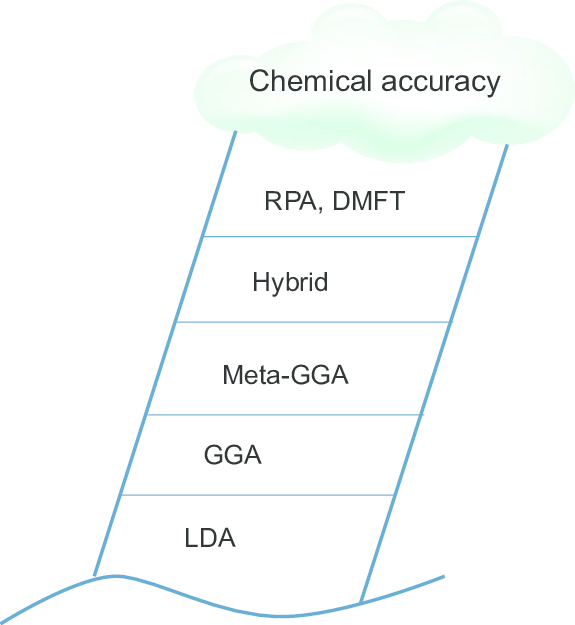
\includegraphics[width=\textwidth,height=\textheight,keepaspectratio]{Figures/jacobs_ladder.png}
    \caption{Jacob's ladder of DFT functionals. \cite{jacobs_ladder}}
    \label{fig:jacobs_ladder}
\end{figure}

\begin{itemize}
    \item \textbf{Local Density Approximation (LDA)}: Depends only on local electron density. It is accurate for uniform electron gases, but less so for molecular systems.
    \item \textbf{Generalized Gradient Approximation (GGA)}: Incorporates density gradients to improve accuracy for molecular and solid-state systems.
    \item \textbf{Meta-GGA Functionals}:  Include kinetic energy density allowing for the capture more detailed electronic effects.
    \item \textbf{Hybrid Functionals}: Combine exact exchange from Hartree-Fock with DFT terms, providing a balance between accuracy and computational cost.
    \item \textbf{Double-Hybrid Functionals}: Incorporate virtual orbital contributions, offering high predictive accuracy.
\end{itemize}

No single functional can describe all systems with equal accuracy. Each functional represents a trade-off between computational cost and precision. The optimal choice depends on the specific system and the properties of interest. 

\subsection{B3LYP functional}

The Becke, three-parameter, Lee-Yang-Parr (B3LYP) hybrid functional is one of the most widely used in computational chemistry. As a hybrid-GGA functional on Jacob’s Ladder, B3LYP incorporates exact exchange from Hartree-Fock (HF) theory. This improves its accuracy over pure DFT approaches by reducing self-interaction errors. B3LYP strikes an effective balance between computational cost and chemical accuracy, making it suitable for a variety of applications, such as structure optimization, reaction energetics, and spectroscopic studies. 

The exchange-correlation energy in B3LYP is given by:

\begin{equation}
    E_{\text{xc}}^{\text{B3LYP}} = (1 - a) E_{\text{x}}^{\text{LDA}} + a E_{\text{x}}^{\text{HF}} + b \Delta E_{\text{x}}^{\text{B88}} + (1 - c) E_{\text{c}}^{\text{LDA}} + c E_{\text{c}}^{\text{LYP}}
\end{equation}

\begin{enumerate}
    \item $E_{\text{x}}^{\text{LDA}}$ and $E_{\text{c}}^{\text{LDA}}$ are the exchange and correlation energy contributions from the Local Density Approximation (LDA).
    \item $E_{\text{x}}^{\text{HF}}$ is the exact exchange energy from Hartree-Fock theory.
    \item $\Delta E_{\text{x}}^{\text{B88}}$ is the gradient-corrected exchange functional developed by Becke (B88).
    \item $E_{\text{c}}^{\text{LYP}}$ is the correlation functional by Lee, Yang, and Parr (LYP).
    \item The parameters $a$, $b$, and $c$ are empirically optimized to improve agreement with experimental data.
\end{enumerate}

B3LYP is effective for geometry optimization, vibrational frequency calculations, thermochemistry, and TD-DFT-based excited-state studies. However, it has several limitations, such as its poor treatment of dispersion interactions and inadequate description of strong correlation effects (e.g., in transition metal complexes). Additionally, it exhibits inaccuracies in long-range charge-transfer excitations due to its incorrect asymptotic exchange behavior. B3LYP functional also tends to over-delocalize electron density in large systems. Despite these limitations, B3LYP remains widely used due to its relatively low computational cost, and many studies have reported results obtained using this functional. 


\subsection{M06-2X functional}

The M06-2X functional, developed by Zhao and Truhlar \cite{Zhao2008}, is a meta-hybrid generalized gradient approximation (meta-hybrid GGA) functional. Designed to improve the description of noncovalent interactions, thermochemistry, and reaction barriers, it is particularly useful when dispersion forces play a significant role. Compared to conventional hybrid functionals, such as B3LYP, M06-2X incorporates a higher fraction of HF exchange (54\%), enhancing its accuracy in describing main-group chemistry and long-range interactions. 

The exchange-correlation energy of M06-2X is expressed as: 

\begin{equation}
    E_{\text{xc}}^{\text{M06-2X}} = E_{\text{x}}^{\text{HF}} + (1 - a) E_{\text{x}}^{\text{GGA}} + a E_{\text{x}}^{\text{Meta-GGA}} + (1 - b) E_{\text{c}}^{\text{GGA}} + b E_{\text{c}}^{\text{Meta-GGA}}
\end{equation}

where:
\begin{enumerate}
  \item $E_{\text{x}}^{\text{HF}}$ and $E_{\text{x,LR}}^{\text{HF}}$ is the exact HF exchange,
  \item remaining terms represent exchange and correlation contributions from GGA and meta-GGA components.
  \item The parameters $a$ and $b$ were optimized through extensive benchmarking.
\end{enumerate}

M06-2X provides superior performance for systems dominated by noncovalent interactions and dispersion forces. This makes it valuable for biomolecular simulations, van der Waals complexes, and supramolecular assemblies. It also improves the prediction of reaction barriers and enhances the description of charge-transfer excitations in TD-DFT. The functional performs well in both main-group and organometallic chemistry, yielding improved bond dissociation energies, ionization potentials, and electron affinities. 

However, M06-2X has limitations as well. Its performance with transition metal complexes is inconsistent due to challenges in accurately capturing d-electron correlation. Although the high proportion of HF exchange reduces self-interaction errors, it does not eliminate them entirely. Additionally, M06-2X functional is more computationally demanding than traditional hybrid functionals and may overestimate reaction barriers in systems with strong correlation effects. Double-hybrid functionals (e.g., ωB97X-2) or dispersion-corrected methods (e.g., B3LYP-D3) may be more  accurate in such cases. 


\subsection{$\omega$B97X-D functional}

The ωB97X-D functional is a range-separated hybrid density functionals that incorporates long-range corrected exchange and empirical dispersion corrections. It was developed to overcome the limitations of traditional hybrid functionals in systems where long-range electron correlation and dispersion forces are crucial. Compared to M06-2X, which is a meta-hybrid GGA, ωB97X-D uses an explicit range-separation parameter to treat short- and long-range interactions separately. This approach is particularly well-suited for modeling extended molecular systems, such as PFAS aggregates. 

The exchange-correlation energy in ωB97X-D is expressed as: 

\begin{equation}
    E_{\text{xc}}^{\omega\text{B97X-D}} = E_{\text{x,SR}}^{\text{HF}} + (1 - a)E_{\text{x,SR}}^{\text{DFT}} + E_{\text{x,LR}}^{\text{HF}} + E_{\text{c}}^{\text{DFT}} + E_{\text{disp}}
\end{equation}

where:
\begin{enumerate}
  \item $E_{\text{x,SR}}^{\text{HF}}$ and $E_{\text{x,LR}}^{\text{HF}}$ are short- and long-range Hartree-Fock exchange.
  \item $E_{\text{x,SR}}^{\text{DFT}}$ is the short-range DFT exchange.
  \item $E_{\text{c}}^{\text{DFT}}$ is the DFT correlation energy.
  \item $E_{\text{disp}}$ is the empirical dispersion correction (Grimme's D2 model).
\end{enumerate}

Unlike B3LYP, which uses fixed HF exchange, or M06-2X, which is parameterized for main-group chemistry, ωB97X-D’s range separation improves accuracy for systems dominated by long-range electrostatics and dispersion forces. This makes it particularly well-suited for modeling weakly interacting species, such as PFAS in aqueous environments. It reduces self-interaction errors and delivers consistent performance across a wide range of molecular sizes. 

For PFAS, which feature polar C–F bonds, hydrophobic tails, and strong solvation effects, ωB97X-D offers several key advantages. Its long-range correction enhances the accuracy of hydrogen bonding; the D2 dispersion correction effectively captures noncovalent aggregation and hydrophobic interactions; and the range-separated exchange improves the modeling of charge redistribution at interfaces. Additionally, HF exchange helps mitigate self-interaction errors in PFAS systems involving electron transfer or ionization processes. 

Although ωB97X-D is more computationally demanding than B3LYP, it often achieves faster convergence than M06-2X for large systems, where self-interaction errors can hinder SCF convergence. However, ωB97X-D lacks the meta-GGA flexibility of M06-2X for modeling transition-state barriers.

\section{Computational tools and workflow}

 The initial 3D structures were generated in Avogadro \cite{avogadro2012}, using the MMFF94 force field for rapid preliminary geometry optimization \cite{avogadro_mmff94}. These pre-optimized geometries were exported as Gaussian 09 input files and processed on laboratory computers at the University of Gdańsk. Each molecule underwent full geometry optimization and vibrational frequency analysis in an aqueous solution using the PCM–SCRF solvation model \cite{gaussian_scrf}. A custom Python script was used to parse the Gaussian log files, extract energies and convert the optimized geometries into XYZ format. Solvent-accessible surface area (SASA) was computed with Open Babel \cite{oboyle2011}, and the molecular descriptors LogP and TPSA were estimated using RDKit \cite{rdkit}. The entire workflow produced nine distinct datasets, resulting from the combination of three functionals and three basis sets.

\subsection{Statistical analysis: ANOVA testing}

A two-way analysis of variance (ANOVA) was performed to evaluate the influence of different computational parameters on molecular descriptors. ANOVA is a statistical technique that determines whether there are statistically significant differences between the means of multiple groups by comparing the variance within groups to the variance between groups. In this master’s thesis, ANOVA was applied to assess the effects of the basis set and functional on the values of the calculated descriptors, as well as their interaction \cite{Orosz2022, Kovacs2021}.

\section{Used molecular descriptors}

\subsection{HOMO, LUMO and the HOMO–LUMO Gap}
The energies of the highest occupied molecular orbital (HOMO) and the lowest unoccupied molecular orbital (LUMO), and especially their difference (the gap), provide insight into a molecule’s propensity to participate in electron transfer or reactive processes. A stabilized HOMO (i.e., lower energy) indicates that the molecule is less likely to donate electrons (i.e., harder to oxidize), while a stabilized LUMO (i.e., higher energy) suggests a reduced ability to accept electrons (i.e., harder to reduce). In PFAS research, molecules with larger HOMO-LUMO gaps tend to be more resistant to oxidative or reductive degradation, which correlates with longer environmental or biological half-lives.\cite{EPA2023}.

\subsection{Topological polar surface area}

Topological polar surface area (TPSA) is calculated as the sum of the surface areas contributed by polar atoms, such as oxygen and nitrogen. Higher TPSA is associated with reduced passive membrane permeability, which may lower absorption but also slow distribution into nonpolar tissues. TPSA also influences elimination and protein binding, especially in PFAS, where high polarity affects interactions with serum proteins and clearance rates.\cite{Ryu2024}

\subsection{Dipole moment}

The molecular dipole moment reflects a molecule’s overall polarity and influences its interactions with water and polar biomolecules. PFAS with larger dipole moments tend to bind more strongly to proteins, such as serum albumin. This binding can slow renal clearance and extend the biological half-life of PFAS. \cite{PengXu2024}

\subsection{Octanol–water partition coefficient}

Octanol–water partition coefficient (LogP) describes a compound’s lipophilicity, or its tendency to partition into hydrophobic environments. In PFAS, higher LogP values are linked to greater accumulation in fatty tissues and sediments, resulting in longer biological and environmental half-lives. \cite{Qiu2020}

\subsection{Solvent accessible surface area}

Solvent accessible surface area (SASA) measures the extent of a molecule’s surface accessible to solvents, reflecting its molecular size and shape. Larger or bulkier PFAS typically exhibit greater resistance to enzymatic or microbial degradation and are metabolized more slowly \textit{in vivo}, contributing to increased persistence. In this master’s thesis, SASA values were calculated using a probe radius of 1.4Å to mimic water as the solvent. 

\subsection{Chemical hardness ($\eta$) and chemical softness ($\sigma$)}
Chemical hardness ($\eta$) is defined as half of the HOMO–LUMO gap and quantifies a molecule’s resistance to changes in electron number. The inverse of hardness, softness ($\sigma$), reflects a molecule’s susceptibility to electron exchange. Hard molecules are less reactive and more resistant to degradation pathways, while softer PFAS may react more readily and degrade more quickly.

\subsection{Chemical potential (\(\mu\)) and electrophilicity (\(\omega\))}
Chemical potential (µ), defined as the average of the HOMO and LUMO energies represents a molecule’s tendency to attract electrons. The electrophilicity index (ω), calculated as  \[
\omega = \frac{\mu^2}{2\eta}
\] quantifies a molecule’s ability to accept electrons. These descriptors, along with hardness and softness were calculated for potential use in machine learning models..

\subsection{Total hartree–fock energy}

Total HF energy reflects a molecule's electronic stabilization and serves as a check to ensure geometry optimizations have properly converged. 


%----------------------------------------------------------------------------------------
\clearpage
\section{Data set}

\subsection{Used data}\\
The primary dataset for this thesis is based on the in vivo PFAS toxicokinetic study by Dawson et al. \cite{dataset_source}. This dataset compiles biological half-life measurements structurally diverse PFAS across four mammalian species: human, monkey, rat, and mouse. Additionally, it records sex-specific differences—showing that, for certain PFAS, males exhibit longer half-lives than females. This supports the inclusion of species and sex as biological descriptors in our models.
 
These experimental data were originally used to train a binary/ranked classification model that categorized PFAS into four half-life ranges: <12h, <1 week, <2 months, and >2 months. The structural diversity of the selected PFAS ranging from short- to long-chain, and including both carboxylates and sulfonates enables robust model training and benchmarking of electronic descriptors.

For our work, we retrieved the molecular structures of nine of the studied PFAS, as well as associated species and sex labels, directly from this source. These serve as input for DFT-based descriptor calculation and subsequent machine learning model training.

The classes in the dataset correspond to biological half-life periods as follows:\\

•	Class 1 : < 0.5 day

•	Class 2: < 1 week

•	Class 3: < 2 months

•	Class 4: > 2 months

Distribution of data looks as follows
\begin{figure}[H]
    \centering
    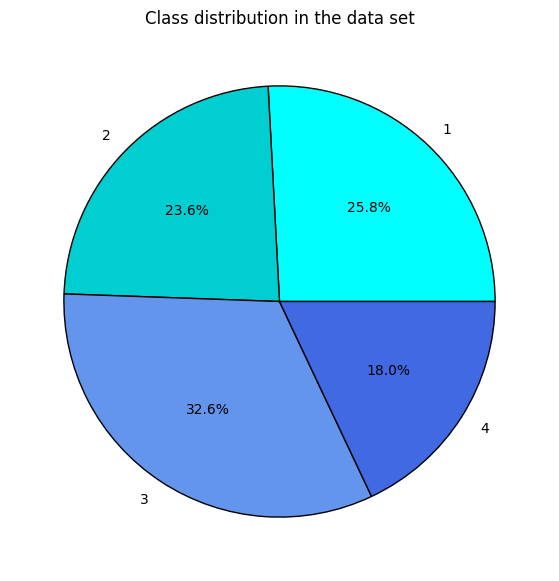
\includegraphics[width=0.5\linewidth]{Figures/classes_pie.png}
    \caption{Class distribution in the dataset}
    \label{fig:class_distribution}
\end{figure}

Figure \ref{fig:class_distribution} shows the distribution of classes within the data set. The number of com- pounds in each class is as follows:\\
•	Class 3: 27 compounds

•	Class 2: 21 compounds

•	Class 4: 16 compounds

•	Class 1: 15 compounds


\subsection{Data division}\\

The data was divided to achieve more balanced classes between the training and validation sets. Six compounds (GenX, Perfluoroheptanoic acid, Perfluorooctanoic acid, Perfluorooctanesulfonic acid, Perfluorobutanesulfonic acid, and Perfluorohexanesulfonic acid) were assigned to the training set, and three compounds (Perfluorononanoic acid, Perfluorobutanoic acid, and Perfluorodecanoic acid) to the validation set. 


Table \ref{tab:train_test_class_distribution} summarizes the distribution of compounds across the training and validation sets


\begin{table}[H]
    \centering
    \caption{Distribution of classes in training and validation set}
    \begin{tabular}{lcc}
         
 class&training set&  validation set\\
         
 3&19&  8\\
         
 2&15&  6\\
         
 4&12&  4\\
          1&11&  4\\
    \end{tabular}
    \label{tab:train_test_class_distribution}
\end{table}

\subsection{Data standarization}
To ensure that the data used in the modeling process are comparable, the next step is to standardize the data set. Standardization is essential because it gives all explanatory variables equal weight, regardless of their original measurement scales or units. Without standardization, accurately interpreting the results would be impossible. Standardization is one of the most widely applied normalization methods. As a result of this process, the data approximate a normal (Gaussian) distribution, which describes how values are distributed around the mean (Figure \ref{fig:gaussian}) \cite{GuhaR}\cite{KumarA}\cite{ZhangX}

\\

\begin{figure}[H]
    \centering
    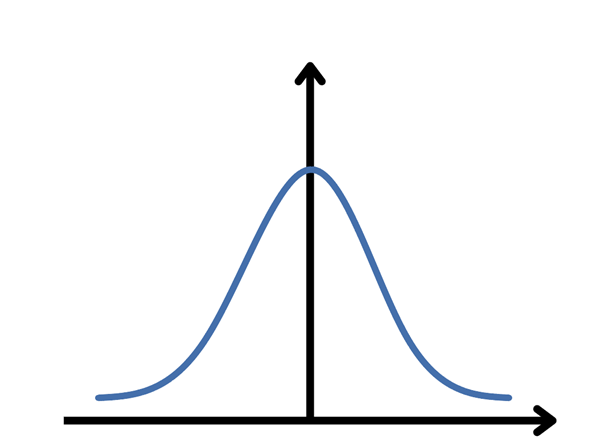
\includegraphics[width=0.5\linewidth]{Figures/image_gausian.png}
    \caption{Normal (Gaussian) distribution. The figure is for illustrative purposes only and does not represent any specific data (own work).}
    \label{fig:gaussian}
\end{figure}

Standardization is defined by the following formula:


\[
\text{z} = \frac{x - u}{\sigma}
\]
where: x - represents the sample value; u - is the mean value for all samples in the column; $\sigma$ - means the standard deviation of all the values in the column\\


In this master's thesis, data standardization was performed using the StandardScaler function from the sklearn.preprocessing library of the Python programming language.\cite{scaler}

\subsection{Feature selection}\\

As illustrated in Figure \ref{fig:heatmap_features} the descriptors were selected based on the correlation matrix, with features showing a correlation coefficient greater than 0.9 being eliminated \cite{heatmap}.

\begin{figure}[H]
    \centering
    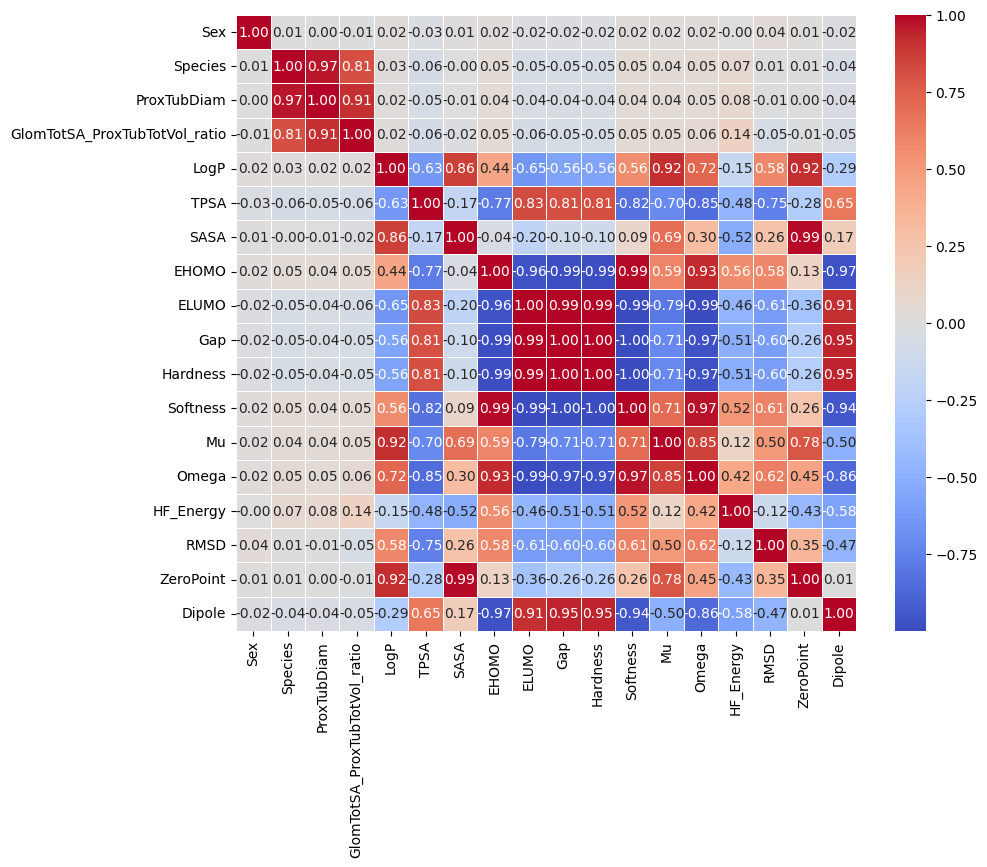
\includegraphics[width=\textwidth,height=\textheight,keepaspectratio]{Figures/matrix_corr.png}
    \caption{Correlation matrix off all features involved in analysis}
    \label{fig:heatmap_features}
\end{figure}

Accordingly, the final set of selected descriptors included the following: Sex, Species, HOMO-LUMO gap, LogP, SASA and HF energy. \textit{’Sex’} and \textit{’Species’} were categorical descriptors extracted from the source article. \cite{dataset_source}

A brief overview of each selected variables is provided below:

\begin{itemize}
    \item \textit{Sex} – This variable included two categories: \textit{‘male’} and \textit{‘female’}, which were encoded numerically as ‘0’ and ‘1’, respectively.
    
    \item \textit{Species} – This categorical variable was also transformed into numerical values: \textit{‘Mice’} = 1; \textit{‘Rats’} = 2; \textit{‘Monkeys’} = 3; and \textit{‘Human’} = 4.

    \item \textit{HOMO-LUMO Gap} – This value represents the energy gap between HOMO and LUMO.
    
    \item \textit{LogP} – This variable reflects lipophilicity, indicating a compound’s ability to dissolve in fats, oils, and nonpolar solvents.
    
    \item \textit{SASA (solvent accessible surface area)} – This molecular descriptor quantifies the surface area of a molecule accessible to a solvent. It reflects the degree to which the molecule is exposed to its surrounding environment.
    
    \item \textit{HF energy (Hartree–Fock energy)} – This descriptor represents a molecule’s total electronic energy, calculated using the Hartree–Fock method, a quantum chemical approach that provides an approximate solution to the Schrödinger equation.
\end{itemize}


\section{Machine learning methods}


\subsection{k - nearest neighbour algorithm}

The k-nearest neighbors (kNN) algorithm is a nonparametric ML method commonly used for classification and regression tasks. It works by measuring the distance between data points, typically using the Euclidean distance, which represents the straight-line distance between two points in a multidimensional space.

The modeling process begins by selecting a value for k, which specifies the number of nearest neighbors to consider. Once k is chosen, a distance matrix is calculated for all data points. Then, the algorithm identifies the k neighbors closest to the data point requiring classification. That data point is then assigned to the class that occurs most frequently among its k nearest neighbors.

For example, if k = 3, the algorithm considers the three nearest neighbors. Number of k is usually an odd number to avoid ties between classes. Suppose the point to be classified lies closest to three other points, two of them belong to class A - represented by a triangle. This class form majority among of nearest neighbors, so the point will be clafiifed as class A - triangle. (Figure \ref{fig:knn_concept}) \cite{HiranK} \cite{ChopraD}

\begin{figure}[H]
    \centering
    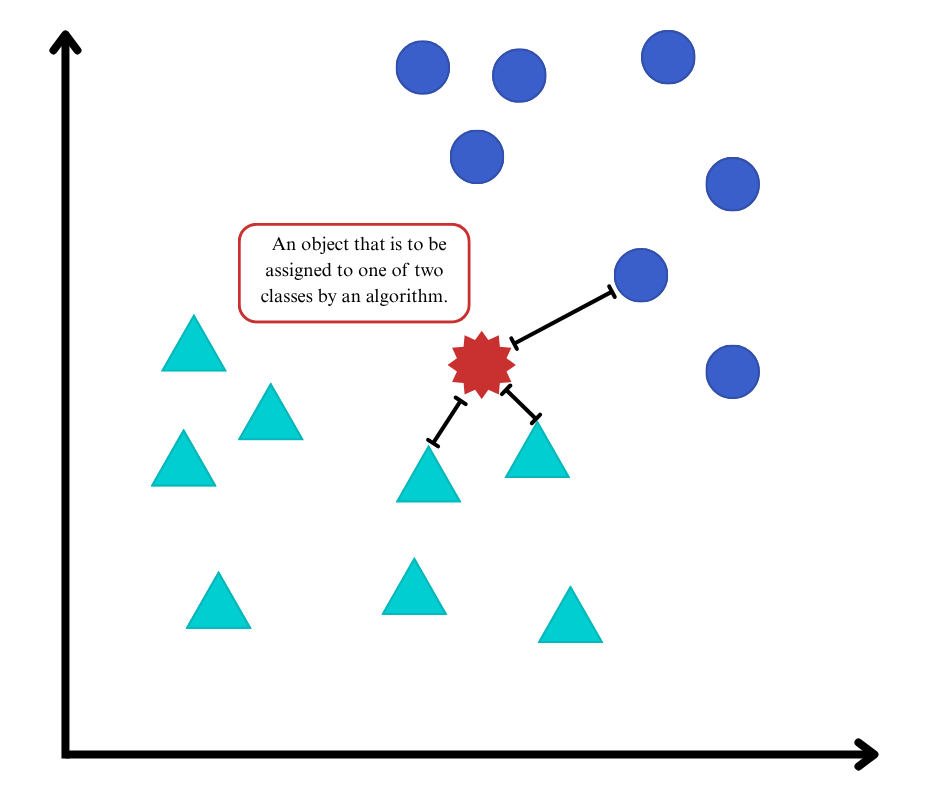
\includegraphics[width=0.5\linewidth]{Figures/knn.png}
    \caption{kNN algorithm concept. The figure is for illustrative purposes
only and does not present any specific data (own work).}
    \label{fig:knn_concept}
\end{figure}



\subsection{Decision trees}

The decision tree (DT) algorithm is a supervised ML method used for classification and regression tasks. One of its major advantages is its simplicity and easy of interpretation because it produces a tree-like diagram. However, the DT algorithm is susceptible to overfitting.

The DT algorithm partitions data along feature axes (Figure \ref{fig:dt_concept}) to accurately separate it by minimizing misclassifications at each split. After the initial division, subsequent splits are performed to further improve class separation. In the example shown, only one object (a circle) is misclassified into the triangle group.

Figure \ref{fig:dt_concept} illustrates this process using a tree structure. In a decision tree classifier, each internal node corresponds to a dataset feature, the branches denote decision rules (i.e., logical rules) based on those features, while the leaf nodes (or leaves) indicate final classification outcomes \cite{HiranK}\cite{ChopraD}.
 
\begin{figure}[H]
    \centering
    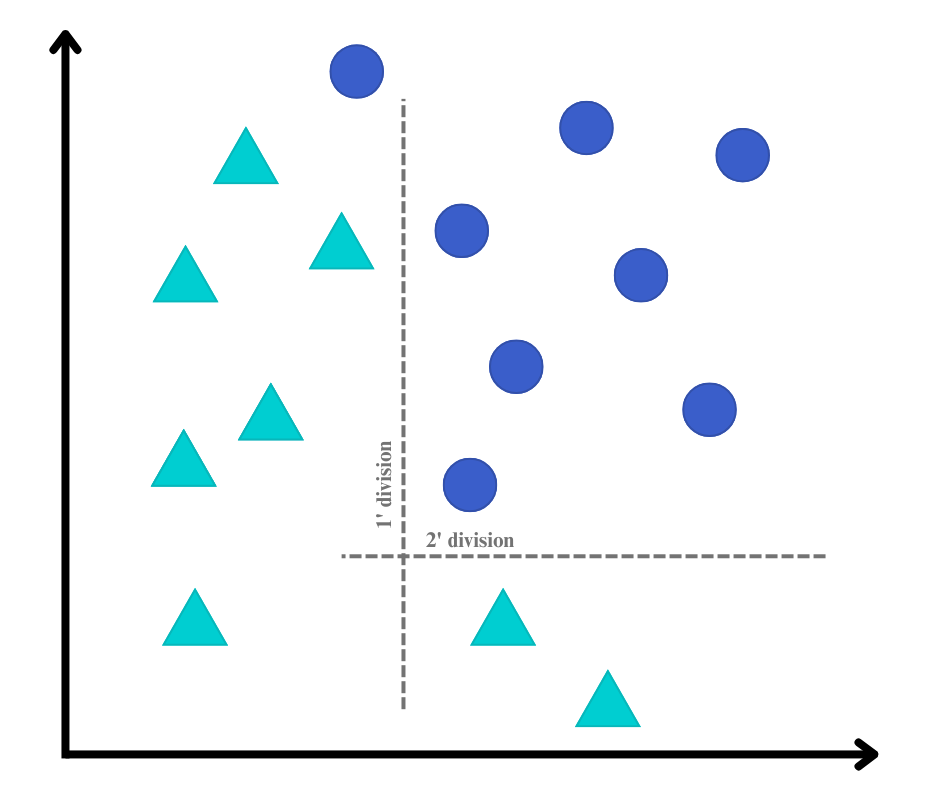
\includegraphics[width=0.5\linewidth]{Figures/DT1.png}
    \caption{The DT algorithm concept. The figure is for illustrative purposes only and does not present any specific data (own work).}
    \label{fig:dt_concept}
\end{figure}

\begin{figure}[H]
    \centering
    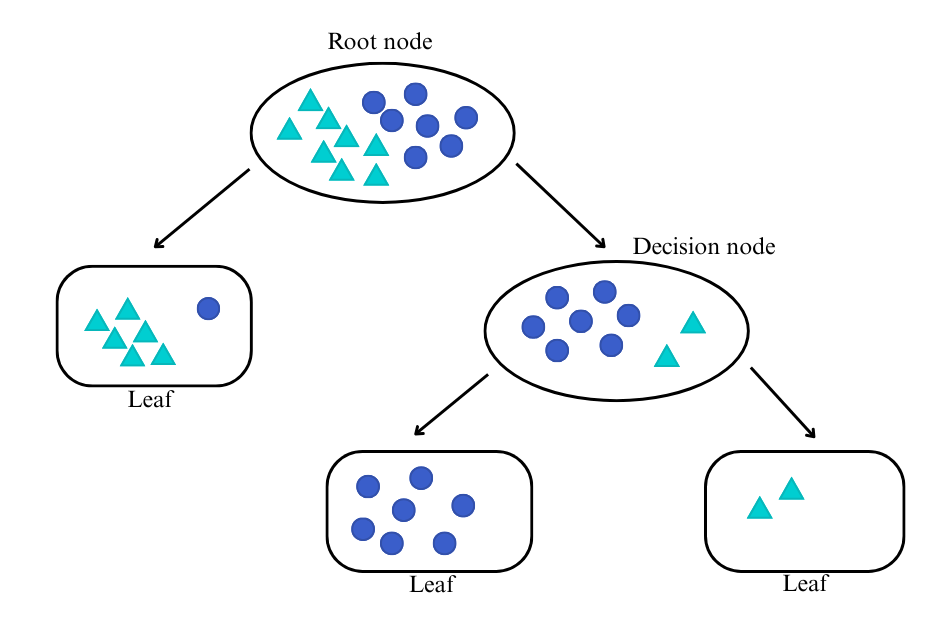
\includegraphics[width=0.5\linewidth]{Figures/DT2.png}
    \caption{The DT algorithm concept. The figure is for illustrative purposes only and does not present any specific data (own work).}
    \label{fig:enter-label}
\end{figure}


\subsection{X- gradient boosting}

XGBoost is an advanced X-gradient boosting algorithm based on DT principles. It generates an ensemble of trees sequentially, where each new tree is trained to correct the prediction errors of the preceding ones, thereby improving the model's overall performance. Despite its high accuracy, XGBoost is prone to overfitting and overtraining, especially if it is not properly regularized. XGBoost can be effectively applied to both regression and classification tasks \cite{Shah}.



\section{Evaluation metrics for classification models}

Classification model performance is assessed using a confusion matrix, which visually summarizes the number of correctly and incorrectly classified instances for each category (Figure \ref{fig:confusion_matrix}) True positive (TP) and true negative (TN) reflect accurate predictions for their respective classes. In contrast, a false positive (FP), also known as a type I error, occurs when the model incorrectly classifies a negative instance as positive. A false negative (FN), also known as a type II error, occurs when a positive instance is incorrectly classified as negative. Of these, false positives are considered more critical than false negatives. For example, in toxicity classification, misclassifying a highly toxicity compound as less toxic poses a greater risk \cite{HiranK}.
 
 
\begin{figure}[H]
    \centering
    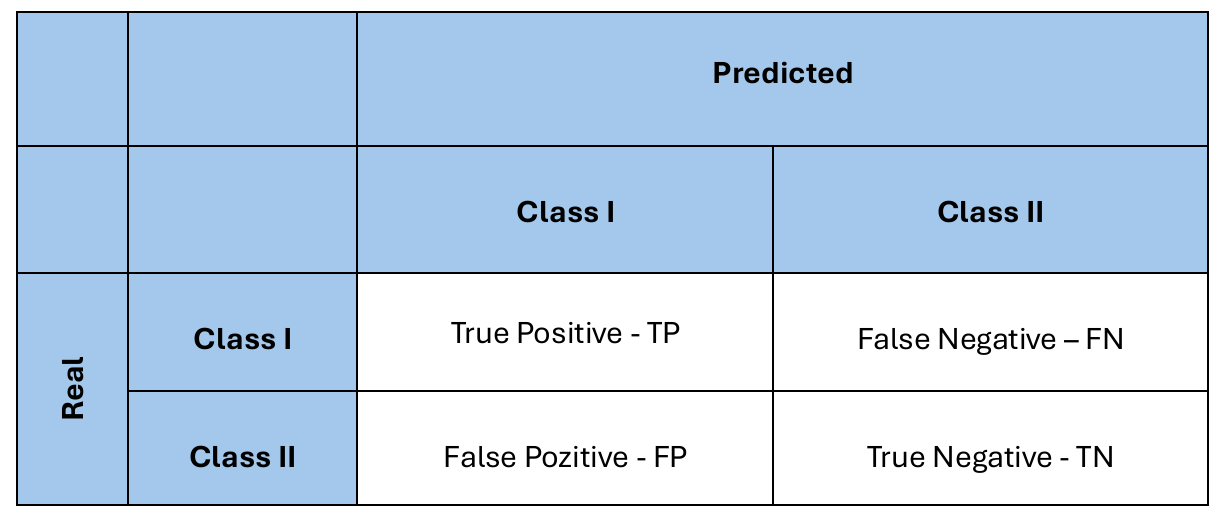
\includegraphics[width=\textwidth,height=\textheight,keepaspectratio]{Figures/matrix_conf.png}
    \caption{Confusion matrix.}
    \label{fig:confusion_matrix}
\end{figure}

The following statistics are commonly calculated using a confusion matrix:\\

I. Accuracy defines the ratio of correctly classified objects to the total number of objects \cite{HiranK}:

\[
\text{Accuracy} = \frac{TP + TN}{TP + TN + FP + FN}
\]\\

\clearpage
II. Precision defines the ratio of correctly classified true positives to all classified positives (i.e., the sum of true positives and false positives) \cite{HiranK}:

\[
\text{Precision} = \frac{TP}{TP + FP}
\]\\

III. Recall defines the ratio of correctly classified true positives to all actual positives (i.e., the sum of true positives and false negatives) \cite{HiranK}:

\[
\text{Recall} = \frac{TP}{TP + FN}
\]\\

IV. Specificity defines the ratio correctly classified true negatives to all actual negatives (i.e., the sum of true negatives and false positives) \cite{HiranK}:
\[
\text{Specificity} = \frac{TN}{TN + FP}
\]\\

V. F1-Score defines the harmonic mean of precision and recall \cite{HiranK}:

\[
\text{F1} = 2*\frac{Precision * Recall}{Precision + Recall}
\]\\


\section{Applicability domain assessment}

In the context of quantitative structure–activity/property relationship [(Q)SAR/QSPR] modeling, evaluating the applicability domain (AD) of a model is an essential step to ensure the reliability of predictions. According to the OECD guidelines for the validation of (Q)SAR models, every model should be accompanied by a clearly defined AD \cite{OECD2004}. The AD is the theoretical chemical space for which the model is expected to make reliable predictions, and compounds outside this domain may lead to extrapolation and reduced predictive accuracy.

Despite the recognized importance of AD assessment in modeling studies, the primary objective of this thesis is not to develop and validate a predictive model. Rather, the goal is to investigate the influence of various quantum-chemical descriptors computed using different exchange-correlation functionals and basis sets on compound representation and modeling performance. Therefore, in accordance with OECD recommendations, but with consideration of the scope of this work, AD will not be analyzed in detail or used as a filtering or evaluation criterion in this study.
